% ============================================================
% LaTeXの使い方（論文執筆テンプレートの付属資料）
%
% このファイルは論文本体（paper.tex）とは独立した解説用の文書です．
% 論文には含まれませんので，安心してコンパイル・編集して構いません．
% コンパイル方法： latexmk how-to-use-latex.tex
% ============================================================

\documentclass[submit,autodetect-engine,dvipdfmx,platex]{ipsj-mod}

\usepackage{amsmath}
\usepackage{graphicx}       % 画像を挿入できるようにする
\usepackage{wrapfig}        % 図の回り込みを許す
\usepackage{xcolor}         % 文字に色をつけられるようにする
\usepackage{colortbl}       % 表に色をつけられるようにする
\usepackage{booktabs}       % 表に横罫線をつけられるようにする
\usepackage{multirow}       % 複雑な表を書けるようにする
\usepackage{ascmac}         % 枠をつけた文を書けるようにする
\usepackage{latexsym}       % 扱える数学記号を追加
\usepackage{bm}             % ベクトル表記を扱えるようにする
\usepackage{array}          % 数式モードで表（や行列）を書けるようにする
\usepackage{hyperref}       % URLをハイパーリンク化する
\usepackage{pxjahyper}      % URLのハイパーリンク化した際の日本語問題を解決する
\usepackage[utf8]{inputenc} % for a UTF8 editor only

% hyperrefが\cite番号をリンク化するとipsjクラスの引用番号ソート処理と衝突するため，
% \bibciteを標準の定義（番号のみを保存）に戻す．URLや\hrefのリンクは従来どおり有効．
\makeatletter
\def\bibcite#1#2{\@newl@bel{b}{#1}{#2}}
\makeatother


\begin{document}

\title{LaTeXの使い方}

\author{論文執筆テンプレート 付属資料}{Supplement to the Paper Template}{NCU}
\affiliate{NCU}{名古屋市立大学 データサイエンス学部}

\begin{abstract}
本稿は，初めて論文を執筆する学生に向けて，LaTeXの基本的な書き方を解説した資料である．
見出し，段落，書体，箇条書き，図，表，参考文献の引用といった，論文執筆で最低限必要になる項目を扱う．
本稿自体が論文執筆テンプレートと同じスタイルファイルを用いて組版されているため，
本稿のPDFと\texttt{how-to-use-latex.tex}のソースを見比べることで，
「どう書けば，どう組み上がるのか」を確認できる．
\end{abstract}

\begin{jkeyword}
LaTeX，論文執筆，BiBTeX
\end{jkeyword}

\maketitle


\section{この文書について}
本稿ではLaTeXの使い方をちょっとだけ解説します．
LaTeXは内容とスタイル（見た目）を切り分けて文書を編集することができるソフトウェアです．
コマンドを駆使して，美しい文書を作成することができます．

本稿を読むときは，このPDFと，同じフォルダにある\texttt{how-to-use-latex.tex}を並べて開いてください．
本稿は論文執筆テンプレートと同じスタイルファイルで組版されていますので，
「ソースにこう書くと，論文ではこう出力される」という対応をそのまま確認できます．

なお，LaTeXの環境の準備やテンプレートのファイル構成については，
1つ上のフォルダにある\texttt{README.md}を参照してください．
また，LaTeXの使い方については様々な書籍，ウェブサイトが解説を行っています．
より詳しい使い方についてはそちらを参考にしてください．


\section{見出し}
\label{sec:heading}
文章を構造化するには，内容を章別，節別に整理することが重要です．
例えば本稿では，この「第\ref{sec:heading}章 見出し」が章に対応し，
すぐ下の「\ref{sec:heading-example} 節見出しの例」が節に対応します．
LaTeXでは\texttt{section}コマンドを用いることで章見出しを，
\texttt{subsection}コマンドを用いることで節見出しを作成することができます．
実際の使い方については，\texttt{how-to-use-latex.tex}ファイルの中身を覗いてみてください．
本章に対応するLaTeXソースが確認できます．

\subsection{節見出しの例}
\label{sec:heading-example}
この見出しは\texttt{subsection}コマンドで作成しています．
章の中をさらに分けたいときに使います．


\section{段落}
ある文章とある文章を段落で分けたい場合，LaTeXでは文章間に空行を入れることで段落を作ることができます．

この節の第2段落のLaTeXソースを確認してください．
前段落の文章とこの段落の文章との間に空行が設けられていることが確認できます．

逆に言うと，空行を入れずに改行しただけでは段落は変わりません．
LaTeXのソースでは，1文ごとに改行して書いておくと，
後から文の入れ替えや修正がしやすくなるのでおすすめです．


\section{書体}
LaTeXではコマンドを用いて，文章の特定の箇所の書体を変更することができます．
例えばこの文書は地の文のデフォルト書体として明朝体が定義されていますが，
\texttt{textgt}コマンドを用いることで，次の1文をゴシック体に変更することができます．

\textgt{このように書体がゴシック体になりました．}

\textgt{ゴシック体}以外にも，{\rm Roman family}，{\tt Typewriter family}，{\sc Small Caps Shape}など，
様々な書体を利用することができます．
どういった書体がどのコマンドで利用できるかは，
\href{http://www.latex-cmd.com/style/style.html}{「LaTeXコマンド集 - 書体」}等のウェブページで確認してください．


\section{文字装飾}
文字を太字にするには\texttt{textbf}コマンドを用います．
文字に下線を引くには\texttt{underline}コマンドを用います．
これらのコマンドを使うことで，このように\textbf{太字}や\underline{下線}で文字を修飾することができます．
実際の使い方については，\texttt{how-to-use-latex.tex}ファイルの中身を覗いてみてください．

なお，学術論文では文字装飾を多用しません．
強調したいことがあるなら，装飾ではなく文章の構成や言葉選びで示すのが基本です．


\section{箇条書き}
箇条書きは番号ありと番号なしの書き方ができます．
番号なしの箇条書きは，
\begin{itemize}
\item 箇条書き1
\item 箇条書き2
\item 箇条書き3
\end{itemize}
のような形式になります．
上記番号なし箇条書きを行うには，以下コードを書きます．
\begin{verbatim}
    \begin{itemize}
        \item 箇条書き1
        \item 箇条書き2
        \item 箇条書き3
    \end{itemize}
\end{verbatim}

番号ありの箇条書きは，
\begin{enumerate}
\item 箇条書きa
\item 箇条書きb
\item 箇条書きc
\end{enumerate}
のような形式になります．
上記番号あり箇条書きを行うには，以下コードを書きます．
\begin{verbatim}
    \begin{enumerate}
        \item 箇条書きa
        \item 箇条書きb
        \item 箇条書きc
    \end{enumerate}
\end{verbatim}


\section{図}

\begin{figure*}[tb]
    \centering
    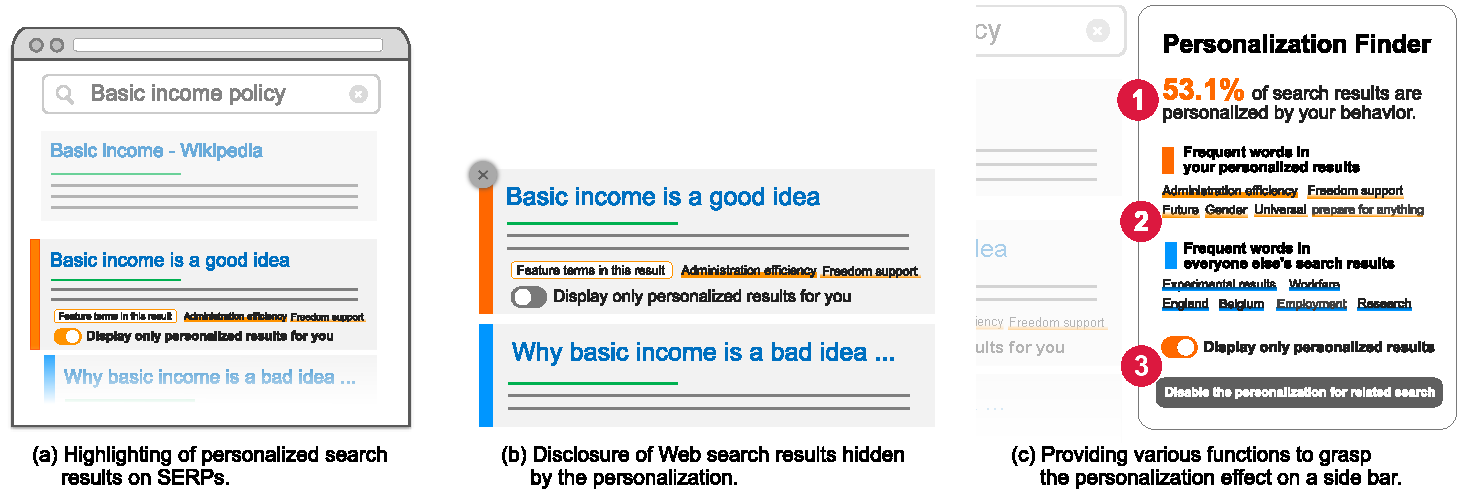
\includegraphics[width=\linewidth]{fig/sample.pdf}
    \caption{図のキャプション}
    \label{fig:example}
\end{figure*}

図を論文に掲載するには\texttt{figure}コマンドおよび\texttt{includegraphics}コマンドを用います．
具体的には以下のようなコマンドを書きます．

\begin{verbatim}
    \begin{figure*}[tb]
        \centering
        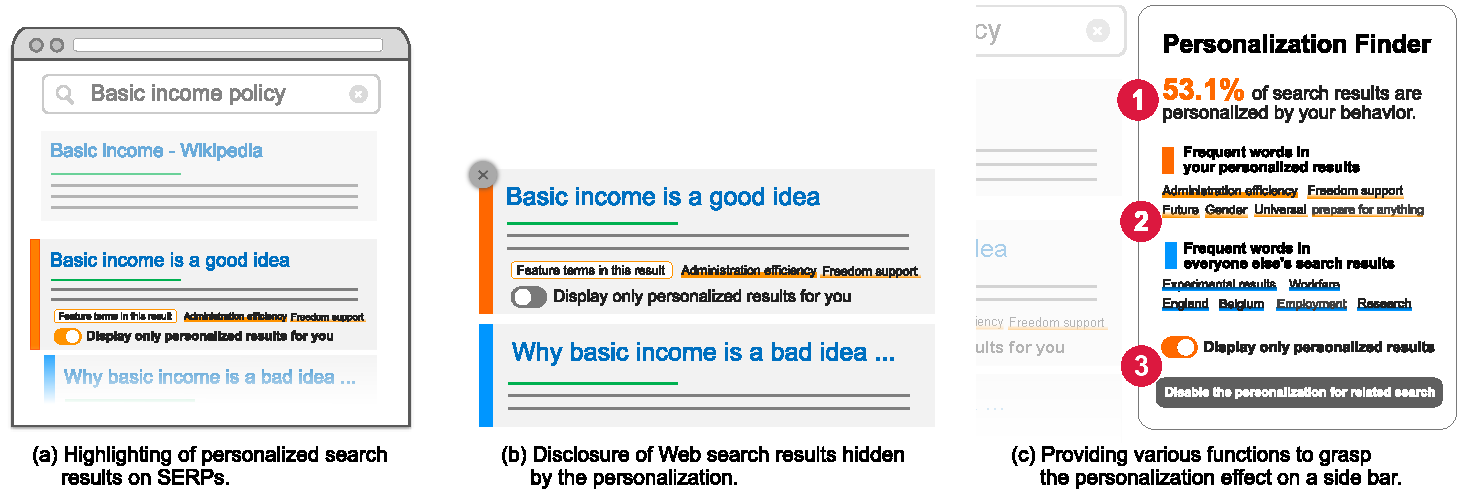
\includegraphics[width=\linewidth]{fig/sample.pdf}
        % 図の幅を直接指定したい場合は以下
        %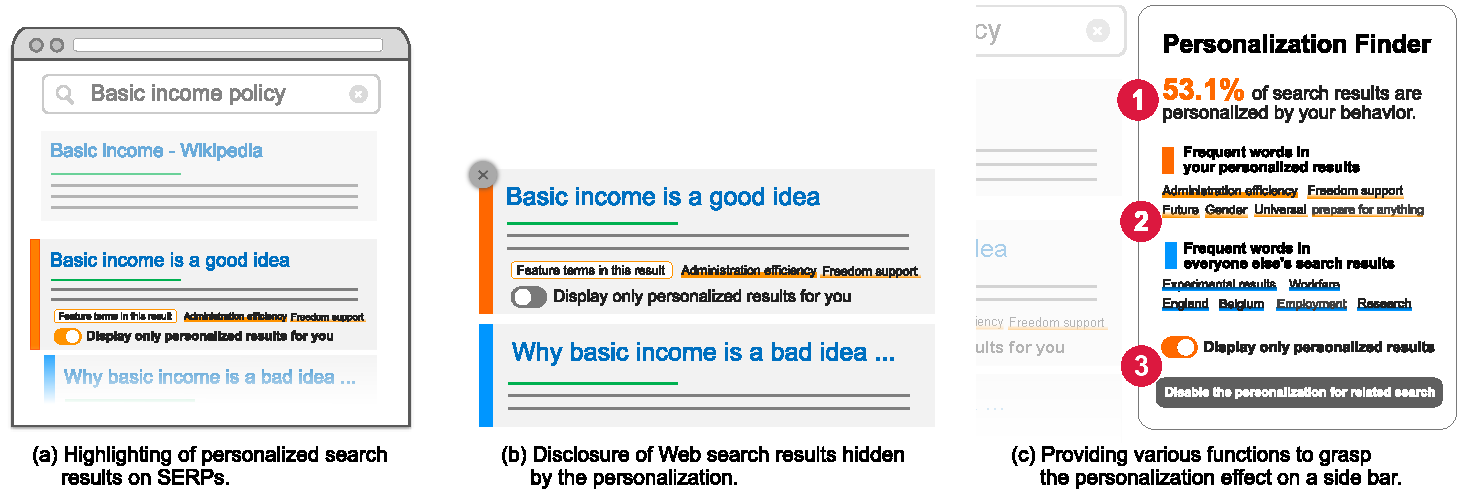
\includegraphics[width=13cm]{fig/sample.pdf}
        \caption{図のキャプション}
        \label{fig:example}
    \end{figure*}
\end{verbatim}
上記コマンドを使うことで，本節で掲載している図を掲載できます．
なお，\texttt{figure}コマンドの代わりに\texttt{figure*}コマンドを用いると，
論文フォーマットが2カラムの場合，2カラム分のスペースを用いて図を掲載します．

LaTeXでは図の配置位置は大まかには指定できますが，ほぼ自動的に行われます．
指定できる位置としては主に「ページ上部（t）」「ページ下部（b）」「図コマンドを挿入した場所（h）」の3種類ありますが，
学術論文ではページ上部もしくはページ下部のどちらかに図を配置することが一般的です．
図の配置位置は\texttt{figure}コマンドのオプションで指定できます．
上の例では図の配置位置のページ上部（優先順位1），ページ下部（優先順位2）を指定しています．

図を掲載するときは図にキャプションを添える必要があります．
キャプションは\texttt{caption}コマンドを用います．

掲載した図（および表）は図表番号を使って論文中で参照します．
論文の修正過程で図表の掲載順を変えた場合，それに応じて本文中の図表参照番号を変更する必要があります（例：図\ref{fig:example}）．
それを逐一手作業で行っていると面倒ですし，誤植の可能性も高まります．
LaTeXではこの問題を解決するために\texttt{label}コマンドを提供しています．
積極的に使いましょう．

なお，図はjpeg画像やpng画像（ラスタ画像）を用いず，PDF化（ベクタ画像化）したものを用いましょう．
ベクタ画像はサイズ変更（例：拡大縮小）が可能ですので，電子的に閲覧する可能性が高い論文ではベクタ画像を用いた方がよいです．


\section{表}
表を論文に掲載するには\texttt{table}コマンドを用います．
具体的には以下のようなコマンドを書きます．

\begin{verbatim}
    \begin{table}[tb]
        \centering
        \caption{被験者の割り当て}
        \scalebox{1.00}{
        \begin{tabular}{c c c}
            \toprule
                & \multicolumn{2}{c}{\textbf{性別}} \\
                \cmidrule(lr){2-3}
            \textbf{UI} & 男性 & 女性 \\
            \midrule
            Type A & 29 & 31 \\
            Type B & 26 & 32 \\
            \bottomrule
        \end{tabular}
        }
        \label{table:example}
    \end{table}
\end{verbatim}
表の配置位置は\texttt{table}コマンドのオプションで指定できます．
上の例では表の配置位置のページ上部（優先順位1），ページ下部（優先順位2）を指定しています．

図のキャプションが図の下に置かれるのに対して，表のキャプションは表の上に置くのが慣例です．
\texttt{caption}コマンドを書く位置に注意してください．
表\ref{table:example}が，上記のコマンドで作成した表です．

\begin{table}[tb]
    \centering
    \caption{被験者の割り当て}
    \scalebox{1.00}{
    \begin{tabular}{c c c}
        \toprule
            & \multicolumn{2}{c}{\textbf{性別}} \\
            \cmidrule(lr){2-3}
        \textbf{UI} & 男性 & 女性 \\
        \midrule
        Type A & 29 & 31 \\
        Type B & 26 & 32 \\
        \bottomrule
    \end{tabular}
    }
    \label{table:example}
\end{table}


\section{参考文献}
参考文献は，LaTeXが提供している\texttt{BiBTeX}という仕組みを利用してください．
\texttt{BiBTeX}とは，一定のルールに基づいて参考文献情報がまとめられたファイルを用意すると，
投稿先が指定した文献フォーマットに従って参考文献リストのフォーマットを整形してくれる仕組みです．
引用したい参考文献は，\texttt{reference.bib}ファイルに書き込みます．
そちらに参考文献情報を書き込み，論文のTeXファイルの中で\texttt{cite}コマンドを用いることで，
\cite{WebSci2018}\cite{Yamamoto2020}のように論文を引用することができます．

なお，\texttt{BiBTeX}用のファイルを用意するのが大変かと思われたかもしれませんが，
ACM Digital LibraryやGoogle Scholarは論文の書誌情報を\texttt{BiBTeX}形式で出力する機能を提供しています．
そちらを有効活用してください．

引用されなかった文献は参考文献リストに載りません．
\texttt{reference.bib}に書いたのにリストに出てこない場合は，
本文中で\texttt{cite}し忘れていないか確認してください．


\bibliography{reference}
\bibliographystyle{ipsjsort}

\end{document}
